\section{Klassen}
%    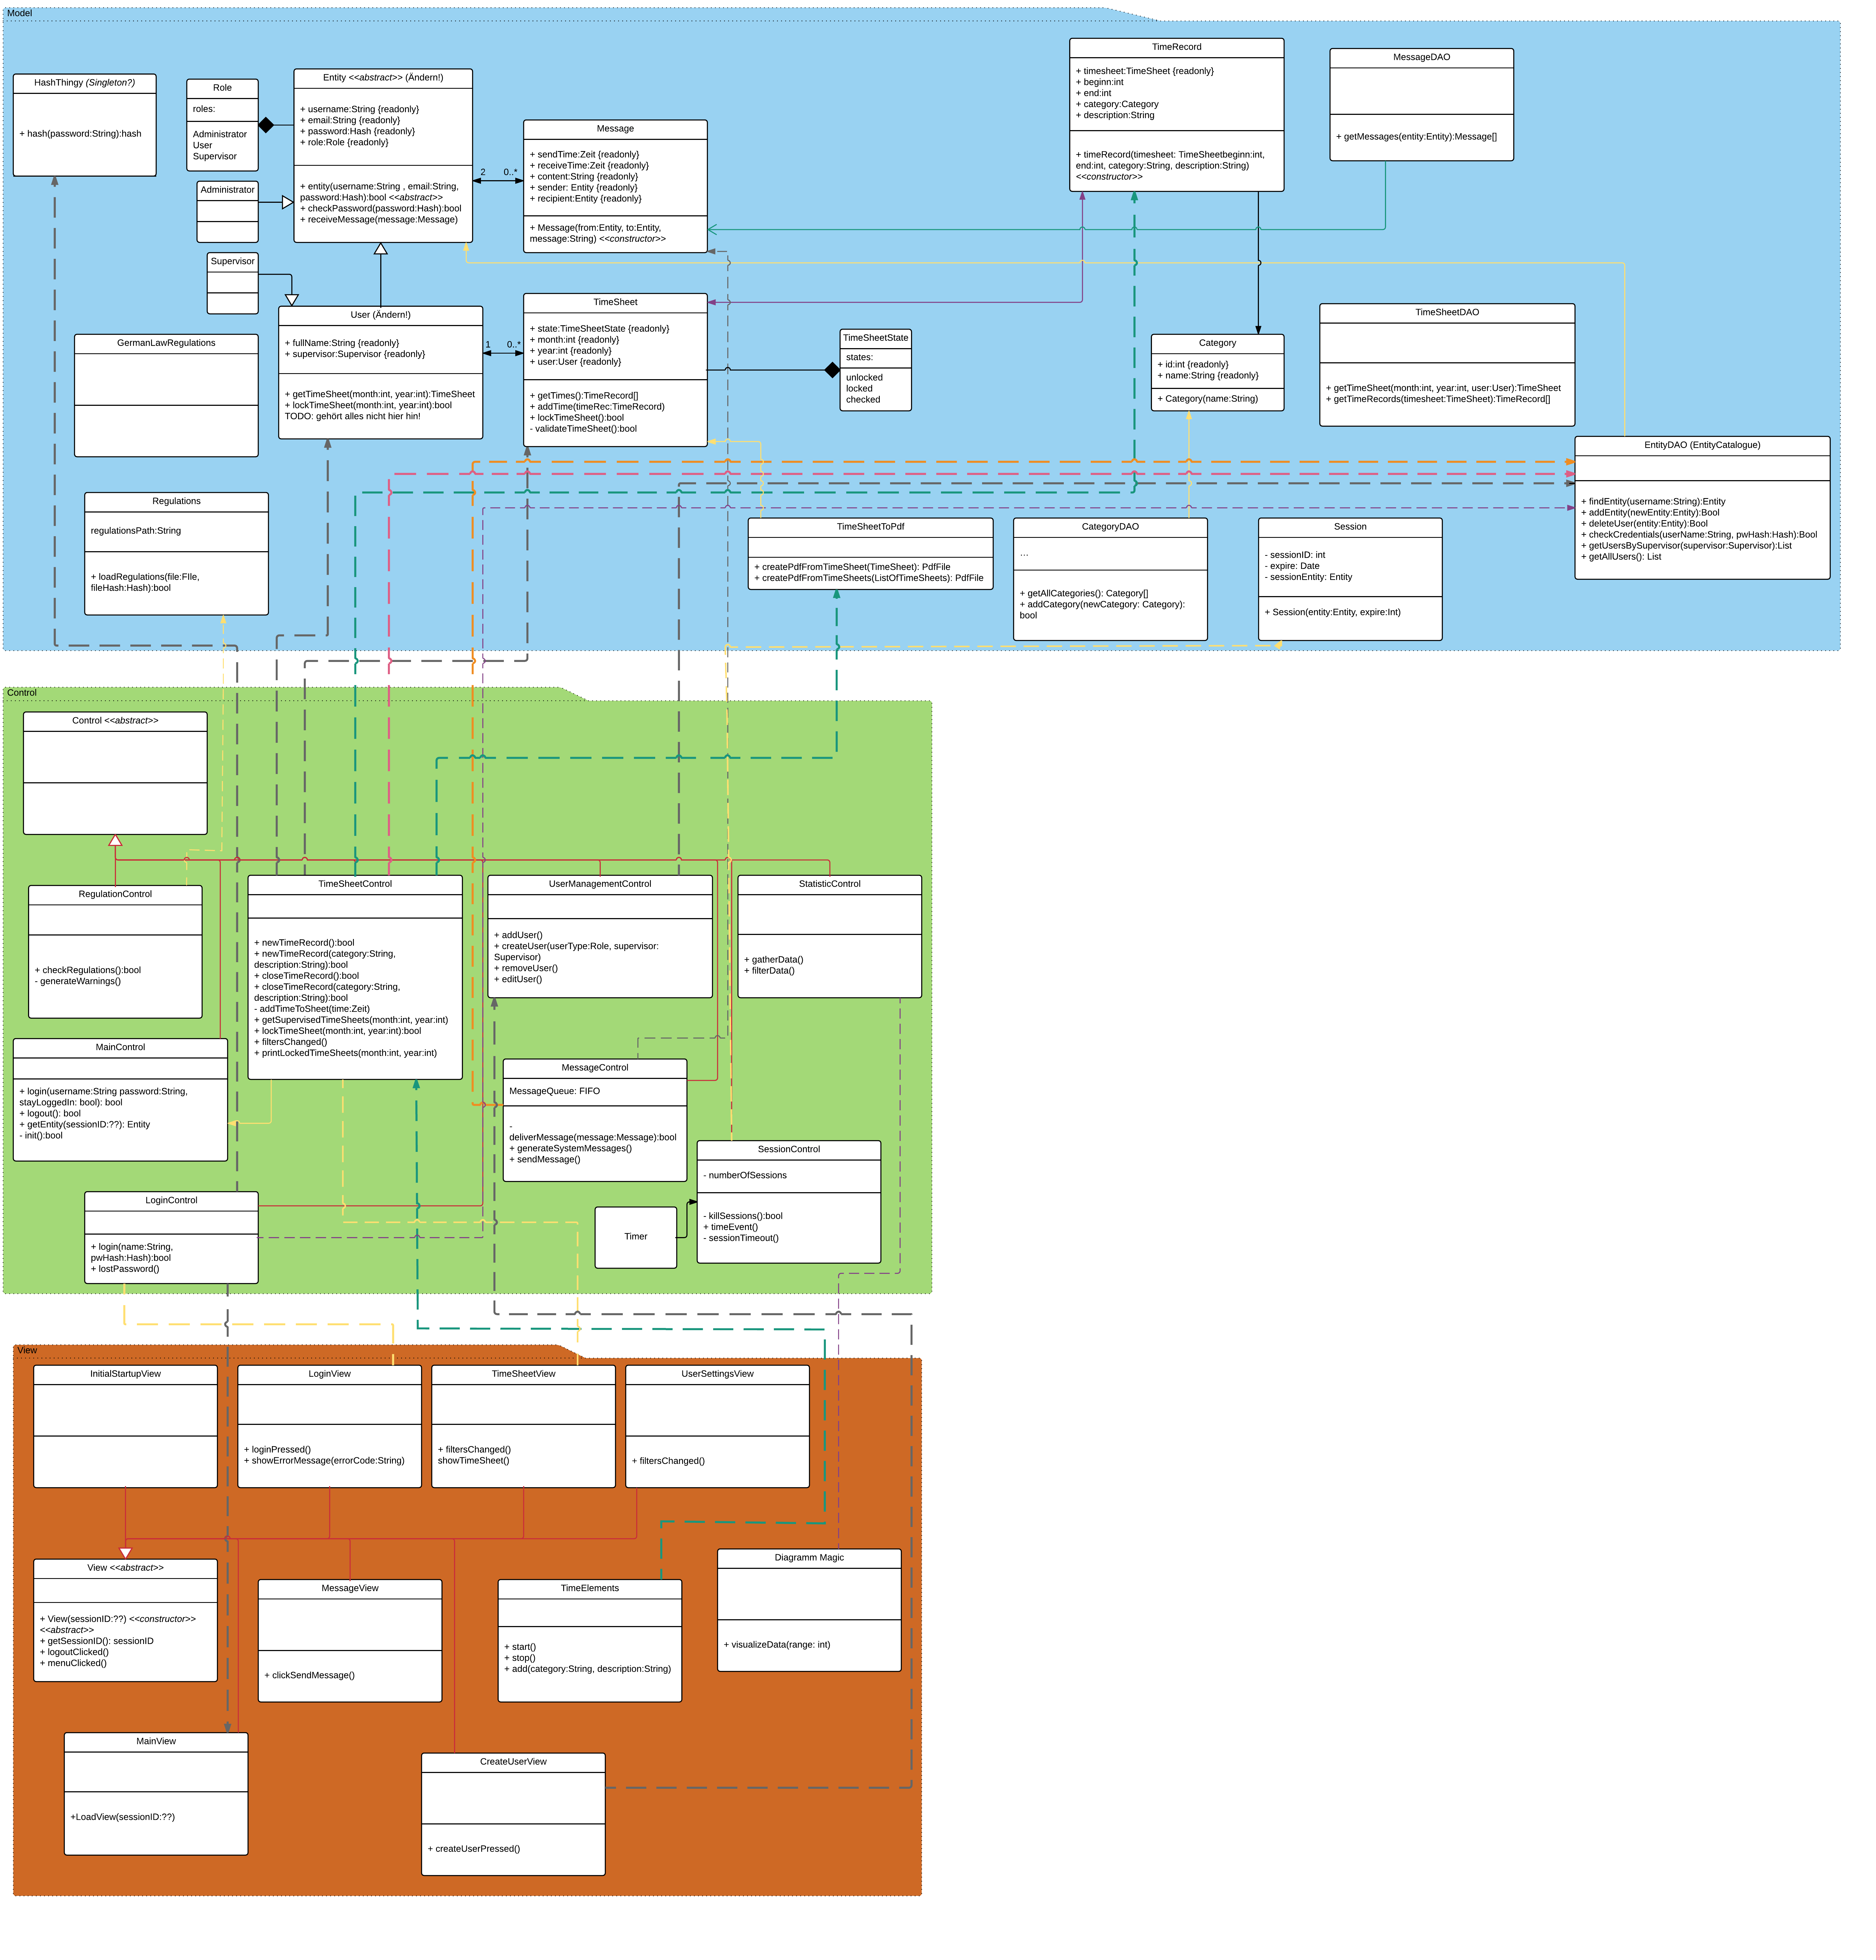
\includegraphics[width=\linewidth]{Diagramms/class/overview.png}\\
    TODO Bild des kompletten Klassendiagrams
    \newpage
    \subsection{Model}
        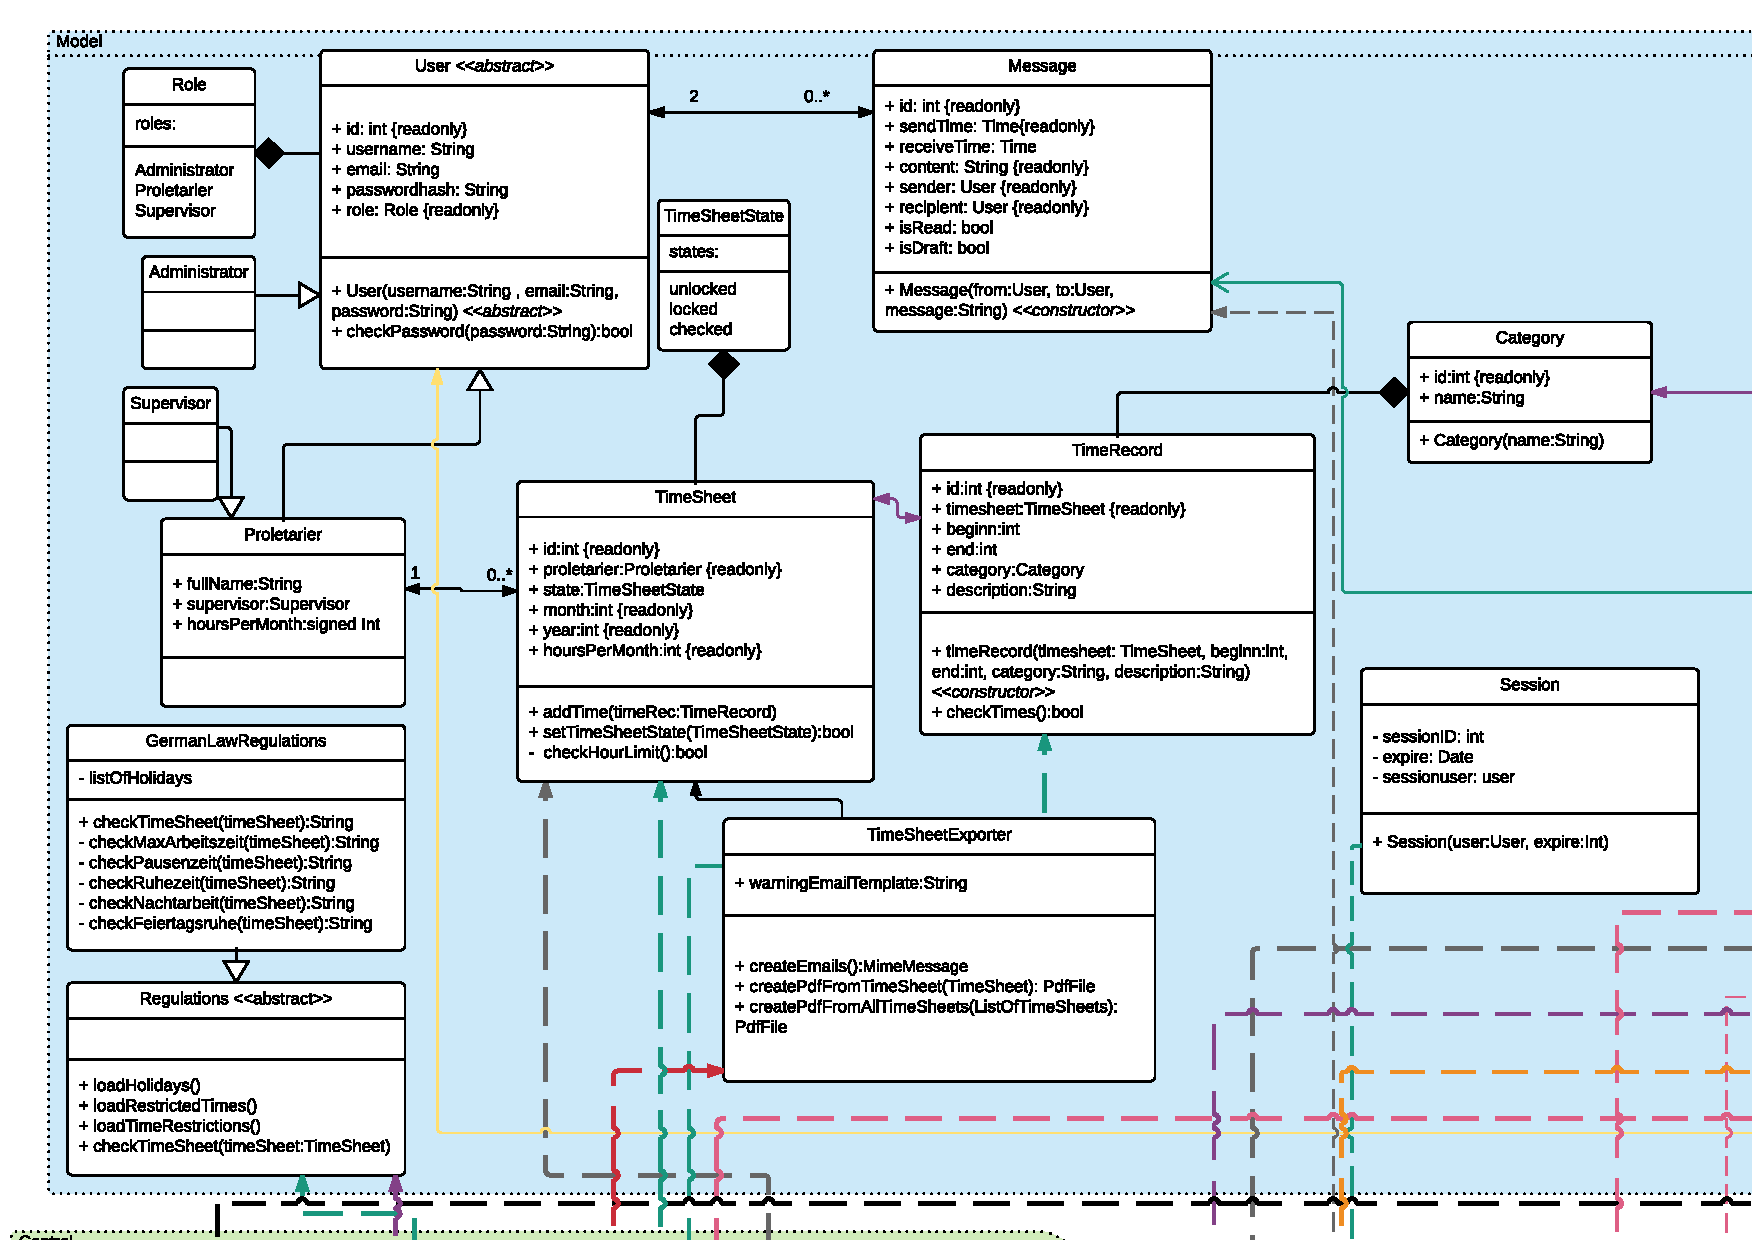
\includegraphics[width=\linewidth,page=1]{Diagramms/class/model.pdf}\\
        \includegraphics[width=\linewidth,page=2]{Diagramms/class/model.pdf}\\
        \begin{itemize}

            \item{User}
                Grundform eines Benutzers, stellt grundlegende Daten und Funktionen für Spezialisierte Benutzer bereit.
                Folgende Spezialisierungen sind möglich:
                \begin{itemize}
                    \item{Admin}
                        Stellt Daten für und über den Admin bereit.
                    \begin{itemize}
                        \item{}
                    \end{itemize}

                    \item{Proletarier}
                        Stellt Daten für und über den Proletarier bereit, darüber hinaus hat der Proletarier eine Verbindung zu dem mit ihm assozierten Zeiterfassungen und Stundenzetteln.
                        \begin{itemize}
                            \item{}
                        \end{itemize}

                    \item{Supervisor}
                        Erweiterung des Proletarier um Gruppen von Usern zu verwalten.
                        \begin{itemize}
                            \item{}
                        \end{itemize}

                \end{itemize}
                \begin{itemize}
                    \item{User\(username:String , email:String, password:Hash\)}
                    \item{checkPassword\(password:Hash\):bool}
                        Gibt true zurück wenn das Passwort korrekt ist sonst false.
                \end{itemize}

            \item{UserDAO}
                Listet alle vorhanden User auf. Enthält Methoden um User hinzuzufügen, zu löschen oder zu verändern. Stellt darüber hinaus sicher, dass die alle Einträge einzigartig sind.
                \begin{itemize}
                   \item{findUser\(username:String\):User}
                   \item{addUser\(newEntity:User\):Bool}
                    Gibt true zurück wenn die User erstellt werden konnte.
                    False bei fehler.
                   \item{deleteUser\(User:User\):Bool}
                    Gibt true zurück wenn die User gelöscht werden konnte.
                    False bei fehler.
                   \item{checkCredentials\(userName:String, pwHash:Hash\):Bool}
                   Gibt true zurück wenn Username und Passwort korrekt sind, sonst false.
                   \item{getUsersBySupervisor\(supervisor:Supervisor\):List}
                   \item{getAllProletarier\(\): List}
                   \item{checkUserDetails(userType:Role, name:String, email:String, password:String, supervisor:Supervisor, hoursPerMonth:int):bool}
                \end{itemize}

            \item{Regulations}
                Lädt die gesetzlichen Regularien aus einer Datei und stellt diese für andere Klassen bereit.
                \begin{itemize}
                    \item{checkTimeSheet\(TimeSheet\):String}
                \end{itemize}

            \item{GermanLawRegulations}
                Lädt die gesetzlichen Regularien aus einer Datei und stellt diese für andere Klassen bereit.
                \begin{itemize}
                    \item{checkTimeSheet\(TimeSheet\):String}
                \end{itemize}

            \item{TimeSheet}
                Speichert Zeiterfassungen. Methoden zur Validierung und sicherstellung der unveränderlichkeit sind vorhanden.
                \begin{itemize}
                    \item{addTime(timeRec:TimeRecord)}
                    \item{setTimeSheetState(TimeSheetState):bool}
                    \item{isLocked():bool}
                    \item{checkHourLimit():bool}
                \end{itemize}

            \item{TimeSheetState}
                Zustände, die beschreiben, ob ein Stundenzettel verändert werden darf, bzw bereits überprüft wurde.
                Mögliche Zustände:
                \begin{itemize}
                    \item{unlocked}
                        Der Time Sheet kann bearbeitet werden.
                    \item{locked}
                        der Time Sheet ist abgeben worden und es deshalb gegen bearbeitung gesperrt.
                    \item{checked}
                        Der Time Sheet wurde vom Supervisor überprüft.
                \end{itemzie}

            \item{TimeSheetHandler}
                \begin{itemize}
                    \item{setTimeSheetState(TimeSheet, TimeSheetState):bool}
                    \item{createPdfFromTimeSheet(TimeSheet): PdfFile}
                    \item{createPdfFromAllTimeSheets(ListOfTimeSheets): PdfFile}
                \end{itemize}


            \item{TimeSheetDAO}
                Listet alle TimeSheets.
                \begin{itemize}
                    \item{getTimeSheet(month:int, year:int, proletarier:Proletarier):TimeSheet}
                    \item{getTimeRecords(timesheet:TimeSheet):TimeRecord[]}
                    \item{getTimeSheetHandler():TimeSheetHandler}
                    \item{getAllUnlockedTimeSheets():List}
                \end{itemize}

            \item{TimeRecord}
                Datenhaltung, der Zeiterfassung.
                \begin{itemize}
                   \item{timeRecord(timesheet: TimeSheetbeginn:int, end:int, category:String, description:String)}
                   \item{checkTimes():bool}
                \end{itemize}

            \item{Session}
                Daten die mit einer Login Session assoziert sind(Proletarier, ablaufdatum, ...) werden in dieser Klasse gespeichert.
                \begin{itemize}
                    \item{Session(User:User, expire:Int)}
                \end{itemize}

            \item{Category}
                Kategorie, die für die Zeiterfassung benötigt wird
                \begin{itemize}
                    \item{Category(name:String)}
                \end{itemize}

            \item{CategorieDAO}
                Liste aller verfügbaren Kategorien.
                \begin{itemize}
                   \item{getAllCategories(): Category[]}
                   \item{addCategory(newCategory: Category): bool}
                \end{itemize}

            \item{Message}
                Nachrichten und damit Verbundene Metadaten können mit dieser Klasse erfasst werden.
                \begin{itemize}
                    \item{Message(from:User, to:User, message:String)}
                \end{itemize}

            \item{MessageDAO}
                Nachrichten und damit Verbundene Metadaten können mit dieser Klasse erfasst werden.
                \begin{itemize}
                    \item{getMessages(user:User):Message[])}
                \end{itemize}


        \end{itemize}

    \subsection{Control}
        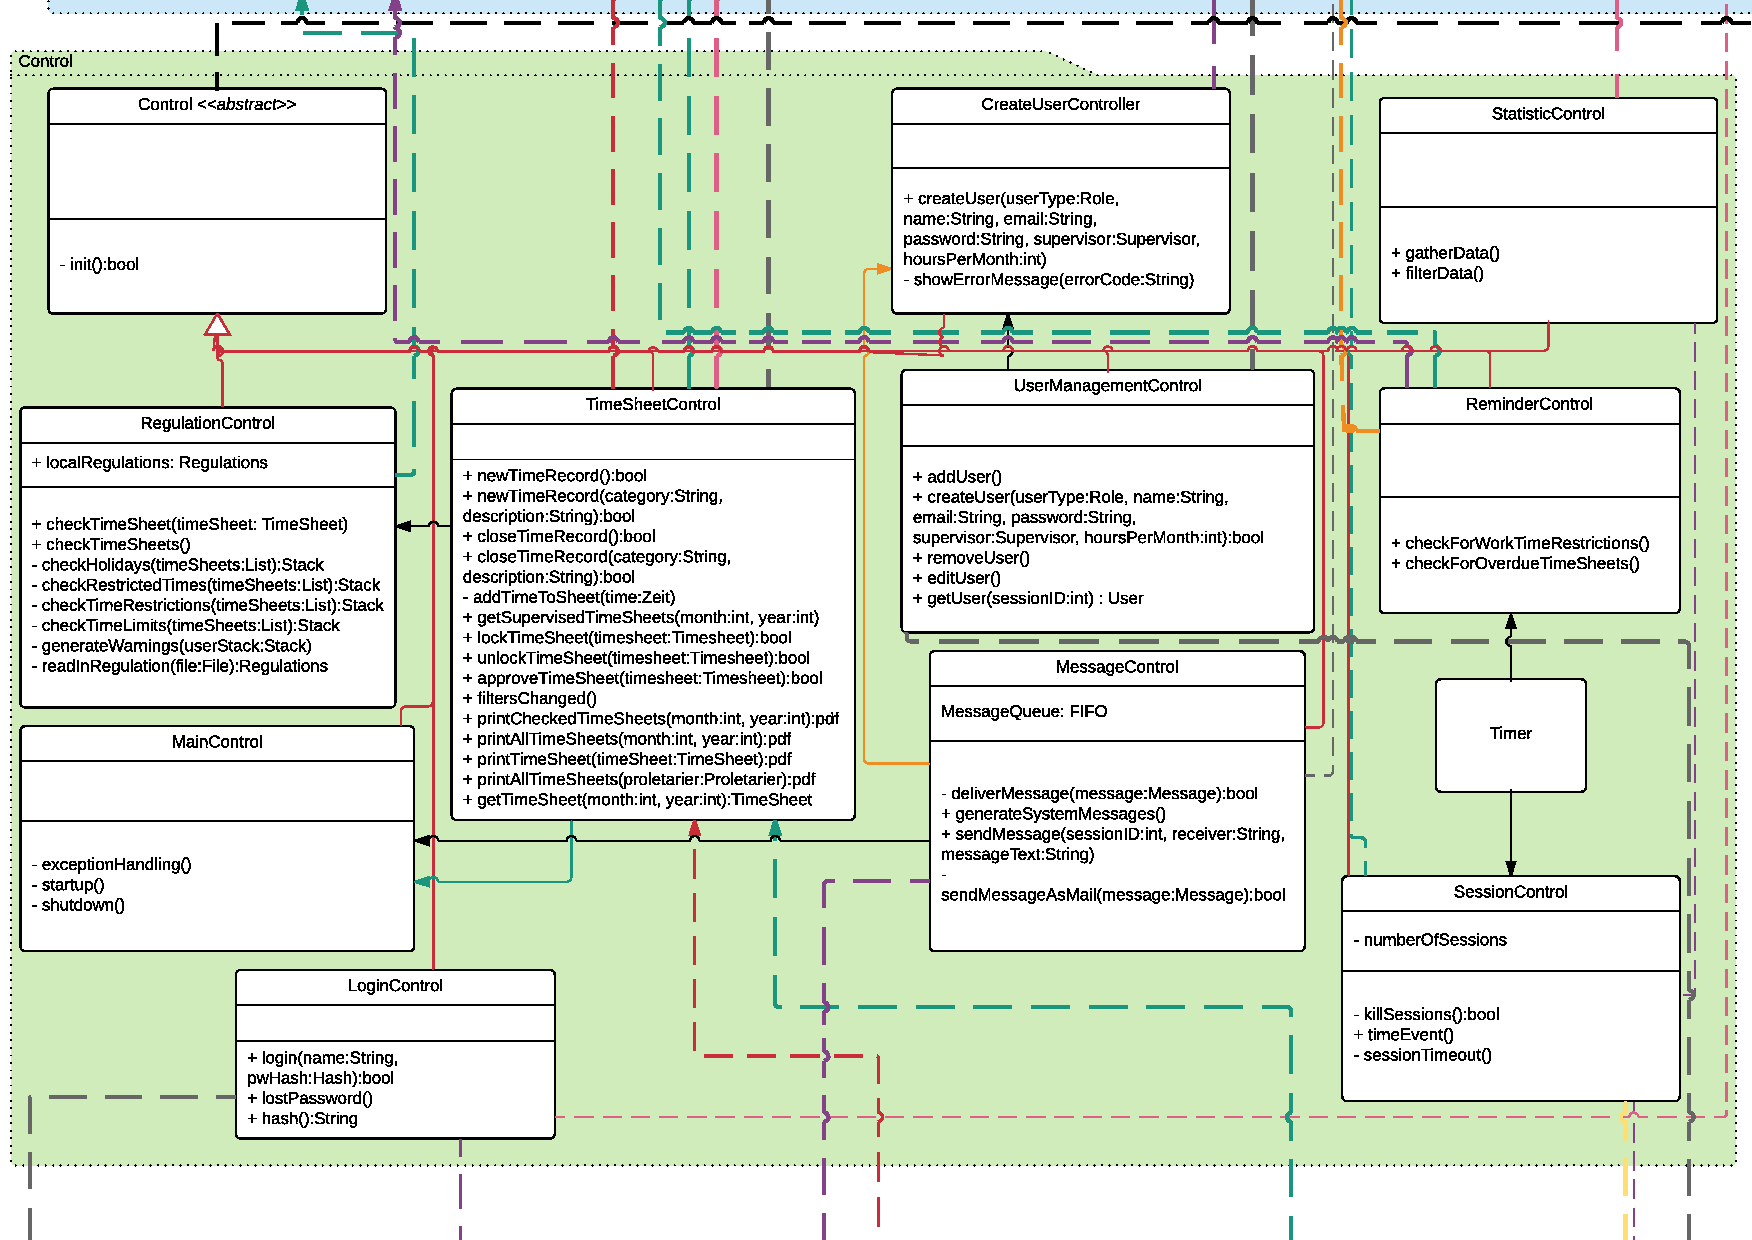
\includegraphics[width=\linewidth]{Diagramms/class/control.pdf}\\
        \begin{itemize}
            \item{Control}
                \begin{itemize}
                    \item{RegulationControl}
                       Überprüft Daten auf Gesetzeskonformität, leitet ebenfalls notwendige Schritte ein.
                       \begin{itemize}
                           \item{checkRegulations():bool}
                            Es werden erfasste Zeiten auf ihre konformität geprüft.
                            \item{checkHolidays(timeSheets:List):Stack}
                            \item{checkRestrictedTimes(timeSheets:List):Stack}
                            \item{checkTimeRestrictions(timeSheets:List):Stack}
                            \item{checkTimeLimits(timeSheets:List):Stack}
                           \item{generateWarnings()}
                            Erzeugt Messages über Verletzungen der Regularien.
                       \end{itemize}

                    \item{MainControl}
                        Kontroliert den Hauptablauf des Programms.
                        \begin{itemize}
                             \item{getEntity(sessionID:??): User}
                             \item{init():bool}
                                Der Server dienst wird initialisiert.
                                False wird zurückgegeben, wenn etwas falsch läuft und die initialisierung fehlschlägt
                        \end{itemize}

                    \item{TimeSheetControl}
                        Regelt die Erstellung von Stundendaten für den Stundenzettel, darüber hinaus wird auch die abrarbeitung eines fertigen Stundenzettels geregelt.
                        \begin{itemize}
                             \item{newTimeRecord():bool}
                             \item{newTimeRecord(category:String, description:String):bool}
                             \item{closeTimeRecord():bool}
                             \item{closeTimeRecord(category:String, description:String):bool}
                             \item{addTimeToSheet(time:Zeit)}
                             \item{getSupervisedTimeSheets(month:int, year:int)}
                             \item{lockTimeSheet(month:int, year:int):bool}
                             \item{filtersChanged()}
                             \item{printLockedTimeSheets(month:int, year:int)}
                             \item{getTimeSheet(month:int, year:int):TimeSheet}
                        \end{itemize}

                    \item{UserManagementControl}
                        Managed das hinzufügen, löschen und verändern von Benutzern
                        \begin{itemize}
                             \item{addUser()}
                             \item{createUser(userType:Role, supervisor: Supervisor)}
                             \item{removeUser()}
                             \item{editUser()}
                             \item{getUser(sessionID:int): User}
                        \end{itemize}

                    \item{LoginControl}
                        Überwacht das korrekte Einloggen von Benutzern.
                        \begin{itemize}
                             \item{login(name:String, pwHash:Hash):bool}
                             \item{lostPassword()}
                             \item{hash():String}
                        \end{itemize}

                    \item{MessageControl}
                        Stellt Nachrichten zwischen Benutzern (und dem System) zu.
                        \begin{itemize}
                             \item{deliverMessage(message:Message):bool}
                             \item{generateSystemMessages()}
                             \item{sendMessage()}
                             \item{sendMessageAsMail(message:Message):bool}
                        \end{itemize}

                    \item{StatisticControl}
                        Sammelt und generiert Statistiken über die erfassten Stundendaten.
                        \begin{itemize}
                             \item{gatherData()}
                             \item{filterData()}
                        \end{itemize}

                    \item{SessionControl}
                        Kontrolliert offene Sessions und terminiert diese nach ablauf eines gesetzen Zeitraums.
                        \begin{itemize}
                            \item{killSessions():bool}
                            \item{timeEvent()}
                            \item{sessionTimeout()}
                        \end{itemize}
                \end{itemize}
                \begin{itemize}
                     \item{}
                \end{itemize}

            \item{Timer}
            \begin{itemize}
                 \item{}
            \end{itemize}

        \end{itemize}

    \subsection{View}
    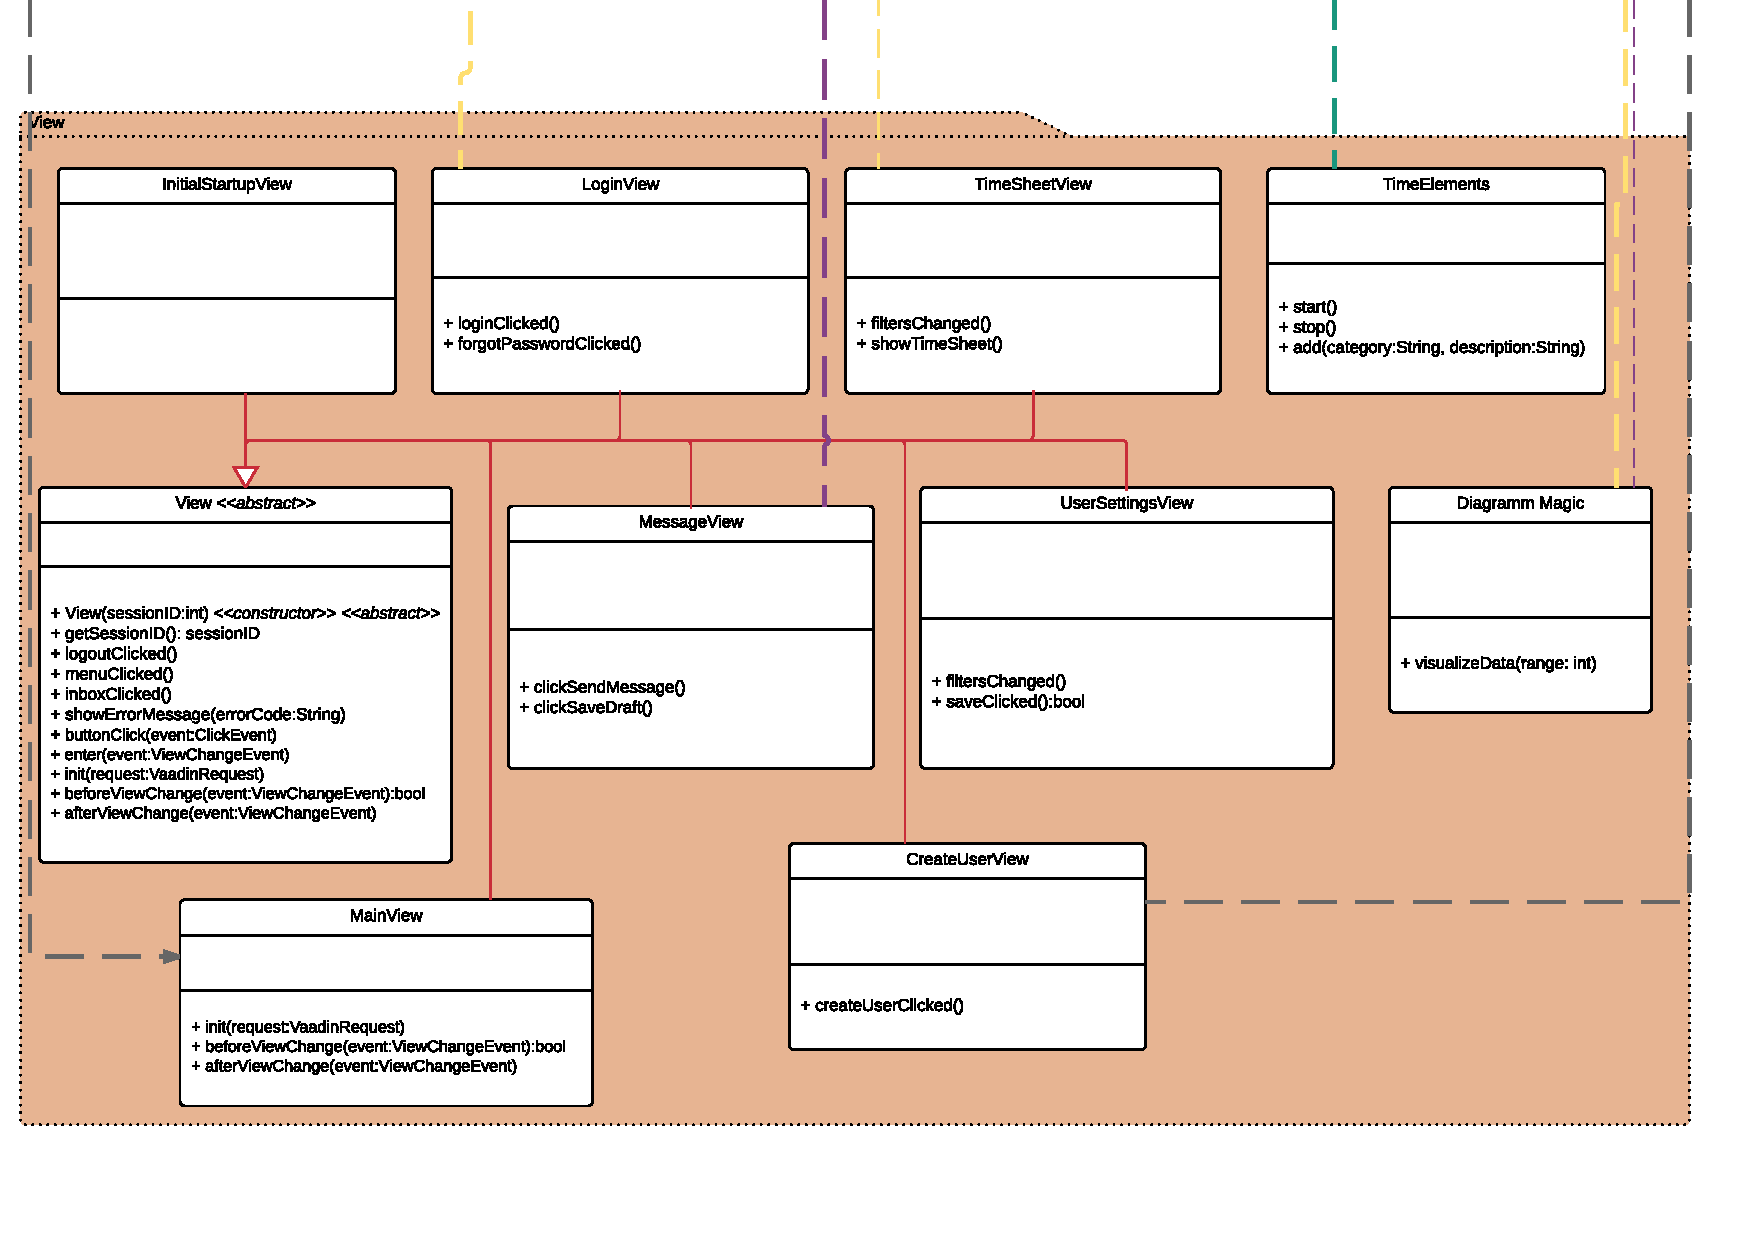
\includegraphics[width=\linewidth]{Diagramms/class/view.pdf}\\
        \begin{itemize}
            \item{View}
                \begin{itemize}
                    \item{LoginView}
                    \begin{itemize}
                        \item{loginPressed()}
                        \item{showErrorMessage(errorCode:String)}
                    \end{itemize}

                    \item{TimeSheetView}
                    \begin{itemize}
                        \item{filtersChanged()}
                        \item{showTimeSheet()}
                    \end{itemize}

                    \item{UserSettingsView}
                    \begin{itemize}
                        \item{filtersChanged()}
                    \end{itemize}

                    \item{MainView}
                    \begin{itemize}
                        \item{LoadView(sessionID:??)}
                    \end{itemize}

                \end{itemize}
                \begin{itemize}
                    \item{View(sessionID:??)}
                    \item{getSessionID(): sessionID}
                    \item{logoutClicked()}
                    \item{menuClicked()}
                \end{itemize}

            \item{Diagramm Magic}
            \begin{itemize}
                \item{visualizeData(range: int)}
                    Zeigt die daten aus der StatisticControl an.
            \end{itemize}

            \item{TimeElements}
            \begin{itemize}
                \item{start()}
                \item{stop()}
                \item{add(category:String, description:String)}
            \end{itemize}

        \end{itemize}